\section{Detailed control design for agreed plant section}
\label{sec:subsec}

\subsection{Control objectives}

\subsection{Key control loops}

\subsubsection{Reactor R201 temperature control}
\begin{figure}[H]
    \centering
    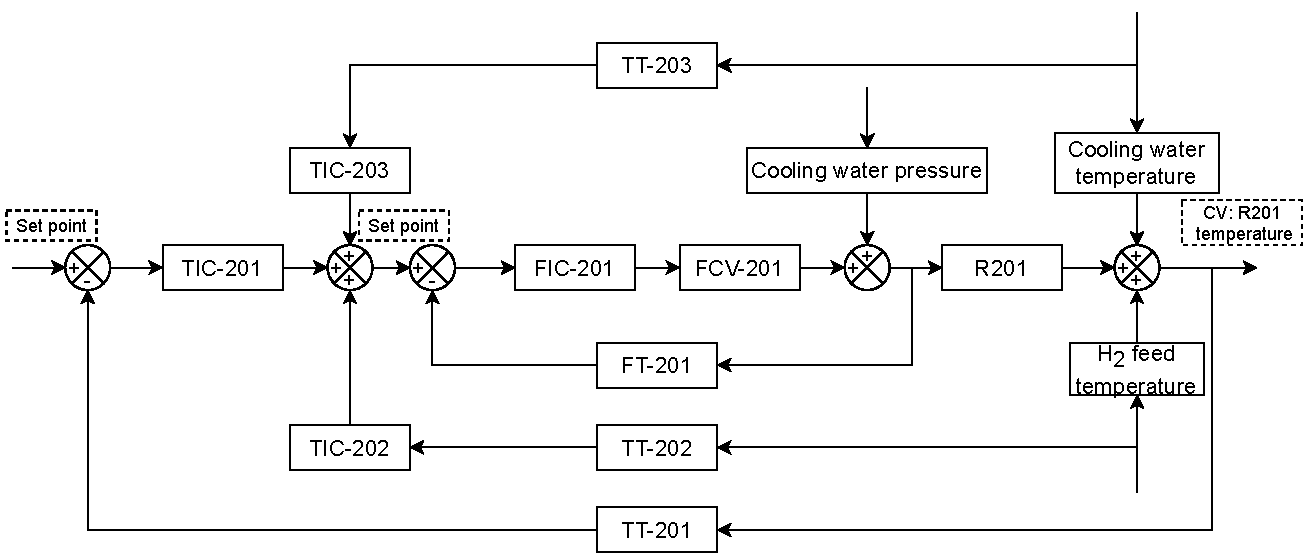
\includegraphics[width=\linewidth]{chapters/4-operation-control/4-Figures/R201-TC.pdf}
    \caption{}
    \label{fig:R201-TC}
\end{figure}

\subsubsection{Reactor R201 pressure control}
\begin{figure}[H]
    \centering
    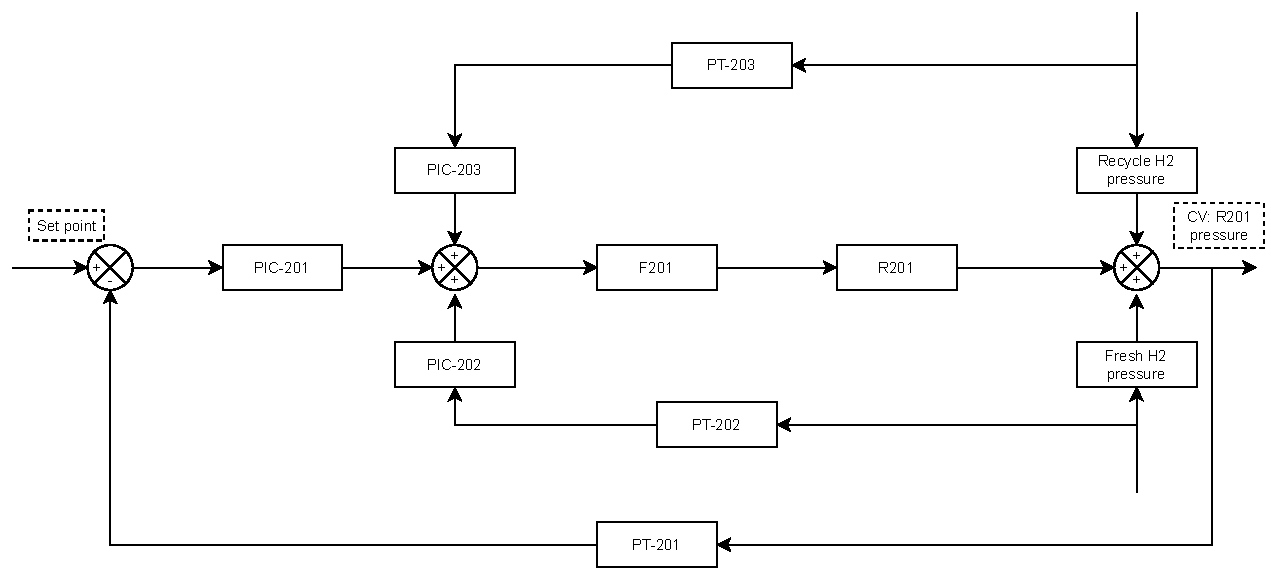
\includegraphics[width=\linewidth]{chapters/4-operation-control/4-Figures/R201-PC.pdf}
    \caption{}
    \label{fig:R201-PC}
\end{figure}

\subsubsection{Reactor R201 level control}
%\begin{figure}[H]
 %   \centering
  %  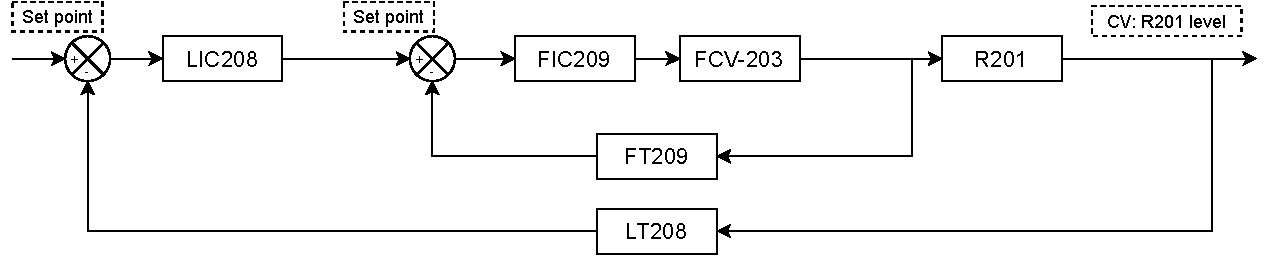
\includegraphics[width=\linewidth]{chapters/4-operation-control/4-Figures/R201-LC.pdf}
   % \caption{}
    %\label{fig:R201-LC}
%\end{figure}

\subsubsection{Reactor feed temperature control}

\subsubsection{Hydrogen recycle control}
\begin{figure}[H]
    \centering
    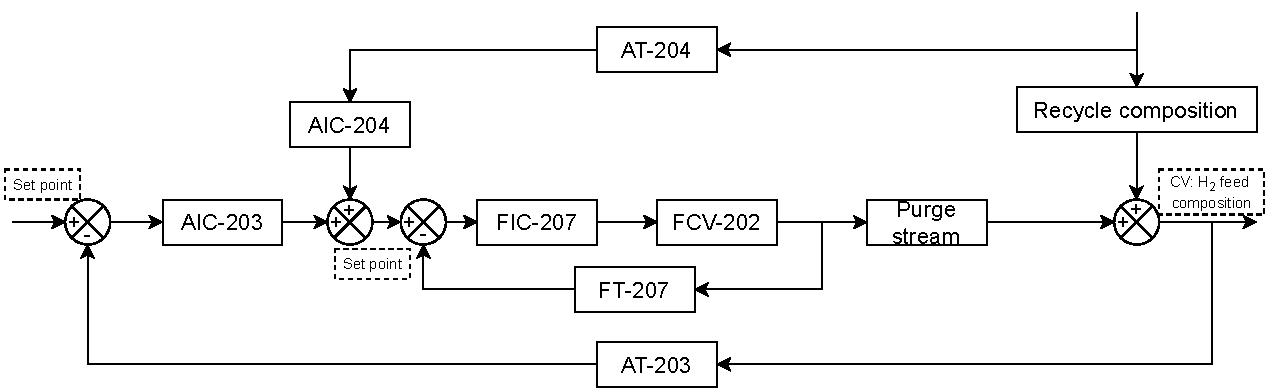
\includegraphics[width=\linewidth]{chapters/4-operation-control/4-Figures/V202-CC.pdf}
    \caption{}
    \label{fig:V202-CC}
\end{figure}

\subsubsection{Reactor outlet flow control}
\begin{figure}[H]
    \centering
    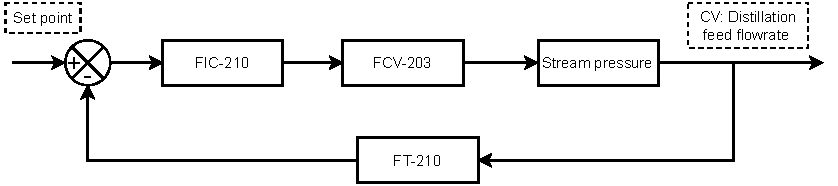
\includegraphics[width=\linewidth]{chapters/4-operation-control/4-Figures/V201-FC.pdf}
    \caption{}
    \label{fig:V201-FC}
\end{figure}


\subsubsection{Control of pressure reduction valve V201}
\begin{figure}[H]
    \centering
    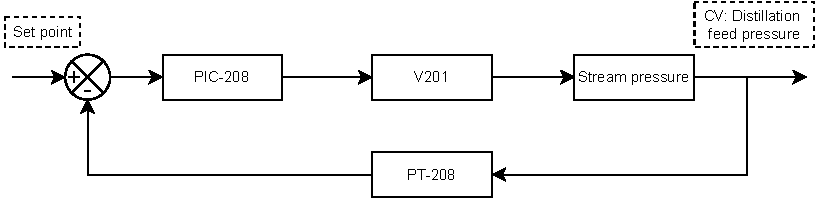
\includegraphics[width=\linewidth]{chapters/4-operation-control/4-Figures/V201-PC.pdf}
    \caption{}
    \label{fig:V201-PC}
\end{figure}

\subsubsection{Distillation column S201 pressure control}
Pressure in distillation columns is regarded as one of the most important parameters to control well, as it not only affects the relative volatilities of the heavy and light keys, but also the shape of the vapour-liquid phase equilibrium curves which determine the compositions of the top and bottoms products of the distillation column. There are several options for for pressure control, such as controlling the vapour flow that is vented from the reflux drum, condenser duty, reboiler duty, recirculation of cooling fluid in the condenser or addition of inerts. Hence the choice of manipulated variable needs to be made carefully considering the relative direct impacts and time delays of each manipulated variable. Controlling the vapour flow that is vented from the reflux drum is the simplest control to implement and usually provides the fastest response as the amount of gas holdup in the column directly affects its pressure. In addition, the vapour flow is large compared . Thus an optimal pressure control strategy was designed with the vapour flowrate from the reflux drum as the manipulated variable. A pressure transmitter (PT 
\begin{figure}[H]
    \centering
    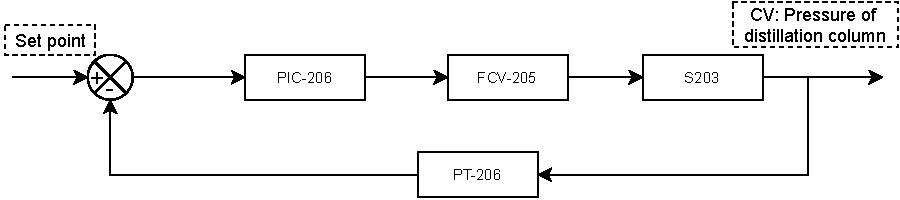
\includegraphics[width=\linewidth]{chapters/4-operation-control/4-Figures/S203-PC.pdf}
    \caption{}
    \label{fig:S203-PC}
\end{figure}

\subsubsection{Distillation column S201 level control}
\begin{figure}[H]
    \centering
    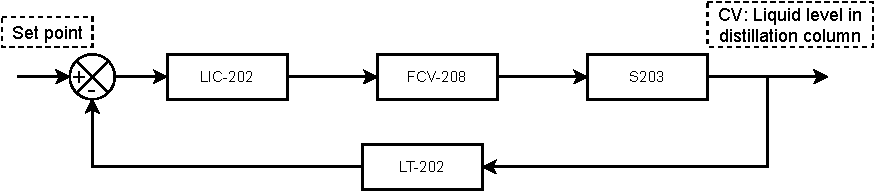
\includegraphics[width=\linewidth]{chapters/4-operation-control/4-Figures/S203-LC.pdf}
    \caption{}
    \label{fig:S203-LC}
\end{figure}

\subsubsection{Bottom stream composition control}
Since the distillation column S201 functions to separate o-toluidine from lighter methanol solvent, it is vitally important to ensure tight composition control in the bottoms stream to maximise the recovery of o-toluidine. 
\begin{figure}[H]
    \centering
    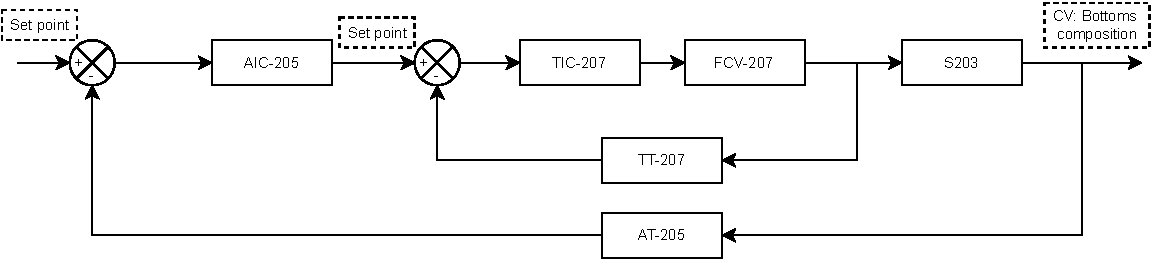
\includegraphics[width=\linewidth]{chapters/4-operation-control/4-Figures/S203-CC.pdf}
    \caption{}
    \label{fig:S203-CC}
\end{figure}

\subsubsection{Reflux drum S204 level control}

\subsubsection{Heat duty of condenser H203 control}
\begin{figure}[H]
    \centering
    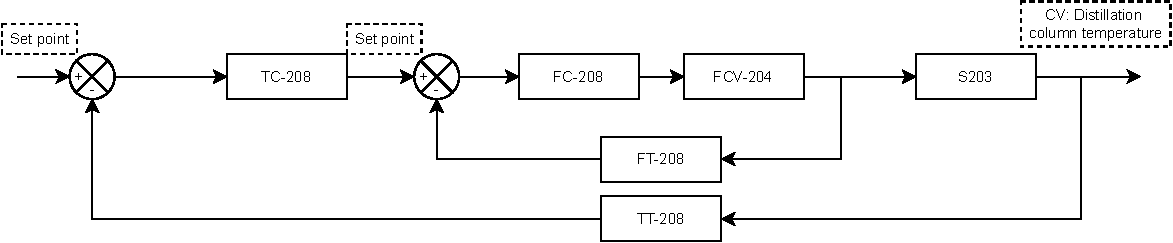
\includegraphics[width=\linewidth]{chapters/4-operation-control/4-Figures/S203C-TC.pdf}
    \caption{}
    \label{fig:S203C-TC}
\end{figure}


\subsubsection{}

\subsection{Safety design}

\subsubsection{Alarms and emergency trips strategy}

\subsubsection{Alarms and safety interlocks design}